\documentclass[1p]{elsarticle_modified}
%\bibliographystyle{elsarticle-num}

%\usepackage[colorlinks]{hyperref}
%\usepackage{abbrmath_seonhwa} %\Abb, \Ascr, \Acal ,\Abf, \Afrak
\usepackage{amsfonts}
\usepackage{amssymb}
\usepackage{amsmath}
\usepackage{amsthm}
\usepackage{scalefnt}
\usepackage{amsbsy}
\usepackage{kotex}
\usepackage{caption}
\usepackage{subfig}
\usepackage{color}
\usepackage{graphicx}
\usepackage{xcolor} %% white, black, red, green, blue, cyan, magenta, yellow
\usepackage{float}
\usepackage{setspace}
\usepackage{hyperref}

\usepackage{tikz}
\usetikzlibrary{arrows}

\usepackage{multirow}
\usepackage{array} % fixed length table
\usepackage{hhline}

%%%%%%%%%%%%%%%%%%%%%
\makeatletter
\renewcommand*\env@matrix[1][\arraystretch]{%
	\edef\arraystretch{#1}%
	\hskip -\arraycolsep
	\let\@ifnextchar\new@ifnextchar
	\array{*\c@MaxMatrixCols c}}
\makeatother %https://tex.stackexchange.com/questions/14071/how-can-i-increase-the-line-spacing-in-a-matrix
%%%%%%%%%%%%%%%

\usepackage[normalem]{ulem}

\newcommand{\msout}[1]{\ifmmode\text{\sout{\ensuremath{#1}}}\else\sout{#1}\fi}
%SOURCE: \msout is \stkout macro in https://tex.stackexchange.com/questions/20609/strikeout-in-math-mode

\newcommand{\cancel}[1]{
	\ifmmode
	{\color{red}\msout{#1}}
	\else
	{\color{red}\sout{#1}}
	\fi
}

\newcommand{\add}[1]{
	{\color{blue}\uwave{#1}}
}

\newcommand{\replace}[2]{
	\ifmmode
	{\color{red}\msout{#1}}{\color{blue}\uwave{#2}}
	\else
	{\color{red}\sout{#1}}{\color{blue}\uwave{#2}}
	\fi
}

\newcommand{\Sol}{\mathcal{S}} %segment
\newcommand{\D}{D} %diagram
\newcommand{\A}{\mathcal{A}} %arc


%%%%%%%%%%%%%%%%%%%%%%%%%%%%%5 test

\def\sl{\operatorname{\textup{SL}}(2,\Cbb)}
\def\psl{\operatorname{\textup{PSL}}(2,\Cbb)}
\def\quan{\mkern 1mu \triangleright \mkern 1mu}

\theoremstyle{definition}
\newtheorem{thm}{Theorem}[section]
\newtheorem{prop}[thm]{Proposition}
\newtheorem{lem}[thm]{Lemma}
\newtheorem{ques}[thm]{Question}
\newtheorem{cor}[thm]{Corollary}
\newtheorem{defn}[thm]{Definition}
\newtheorem{exam}[thm]{Example}
\newtheorem{rmk}[thm]{Remark}
\newtheorem{alg}[thm]{Algorithm}

\newcommand{\I}{\sqrt{-1}}
\begin{document}

%\begin{frontmatter}
%
%\title{Boundary parabolic representations of knots up to 8 crossings}
%
%%% Group authors per affiliation:
%\author{Yunhi Cho} 
%\address{Department of Mathematics, University of Seoul, Seoul, Korea}
%\ead{yhcho@uos.ac.kr}
%
%
%\author{Seonhwa Kim} %\fnref{s_kim}}
%\address{Center for Geometry and Physics, Institute for Basic Science, Pohang, 37673, Korea}
%\ead{ryeona17@ibs.re.kr}
%
%\author{Hyuk Kim}
%\address{Department of Mathematical Sciences, Seoul National University, Seoul 08826, Korea}
%\ead{hyukkim@snu.ac.kr}
%
%\author{Seokbeom Yoon}
%\address{Department of Mathematical Sciences, Seoul National University, Seoul, 08826,  Korea}
%\ead{sbyoon15@snu.ac.kr}
%
%\begin{abstract}
%We find all boundary parabolic representation of knots up to 8 crossings.
%
%\end{abstract}
%\begin{keyword}
%    \MSC[2010] 57M25 
%\end{keyword}
%
%\end{frontmatter}

%\linenumbers
%\tableofcontents
%
\newcommand\colored[1]{\textcolor{white}{\rule[-0.35ex]{0.8em}{1.4ex}}\kern-0.8em\color{red} #1}%
%\newcommand\colored[1]{\textcolor{white}{ #1}\kern-2.17ex	\textcolor{white}{ #1}\kern-1.81ex	\textcolor{white}{ #1}\kern-2.15ex\color{red}#1	}

{\Large $\underline{12n_{0729}~(K12n_{0729})}$}

\setlength{\tabcolsep}{10pt}
\renewcommand{\arraystretch}{1.6}
\vspace{1cm}\begin{tabular}{m{100pt}>{\centering\arraybackslash}m{274pt}}
\multirow{5}{120pt}{
	\centering
	\includegraphics[width=112pt]{../../../GIT/diagram.site/Diagrams/png/2818_12n_0729.png}\\
\ \ \ A knot diagram\footnotemark}&
\allowdisplaybreaks
\textbf{Linearized knot diagam} \\
\cline{2-2}
 &
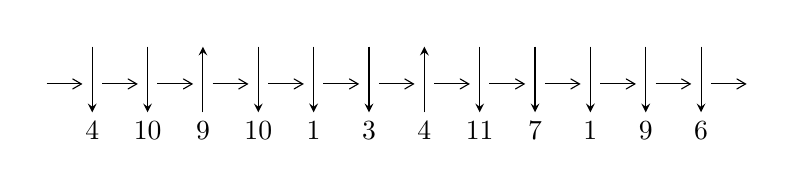
\begin{tikzpicture}[x=20pt, y=17pt]
	% nodes
	\node (C0) at (0, 0) {};
	\node (C1) at (1, 0) {};
	\node (C1U) at (1, +1) {};
	\node (C1D) at (1, -1) {4};

	\node (C2) at (2, 0) {};
	\node (C2U) at (2, +1) {};
	\node (C2D) at (2, -1) {10};

	\node (C3) at (3, 0) {};
	\node (C3U) at (3, +1) {};
	\node (C3D) at (3, -1) {9};

	\node (C4) at (4, 0) {};
	\node (C4U) at (4, +1) {};
	\node (C4D) at (4, -1) {10};

	\node (C5) at (5, 0) {};
	\node (C5U) at (5, +1) {};
	\node (C5D) at (5, -1) {1};

	\node (C6) at (6, 0) {};
	\node (C6U) at (6, +1) {};
	\node (C6D) at (6, -1) {3};

	\node (C7) at (7, 0) {};
	\node (C7U) at (7, +1) {};
	\node (C7D) at (7, -1) {4};

	\node (C8) at (8, 0) {};
	\node (C8U) at (8, +1) {};
	\node (C8D) at (8, -1) {11};

	\node (C9) at (9, 0) {};
	\node (C9U) at (9, +1) {};
	\node (C9D) at (9, -1) {7};

	\node (C10) at (10, 0) {};
	\node (C10U) at (10, +1) {};
	\node (C10D) at (10, -1) {1};

	\node (C11) at (11, 0) {};
	\node (C11U) at (11, +1) {};
	\node (C11D) at (11, -1) {9};

	\node (C12) at (12, 0) {};
	\node (C12U) at (12, +1) {};
	\node (C12D) at (12, -1) {6};
	\node (C13) at (13, 0) {};

	% arrows
	\draw[->,>={angle 60}]
	(C0) edge (C1) (C1) edge (C2) (C2) edge (C3) (C3) edge (C4) (C4) edge (C5) (C5) edge (C6) (C6) edge (C7) (C7) edge (C8) (C8) edge (C9) (C9) edge (C10) (C10) edge (C11) (C11) edge (C12) (C12) edge (C13) ;	\draw[->,>=stealth]
	(C1U) edge (C1D) (C2U) edge (C2D) (C3D) edge (C3U) (C4U) edge (C4D) (C5U) edge (C5D) (C6U) edge (C6D) (C7D) edge (C7U) (C8U) edge (C8D) (C9U) edge (C9D) (C10U) edge (C10D) (C11U) edge (C11D) (C12U) edge (C12D) ;
	\end{tikzpicture} \\
\hhline{~~} \\& 
\textbf{Solving Sequence} \\ \cline{2-2} 
 &
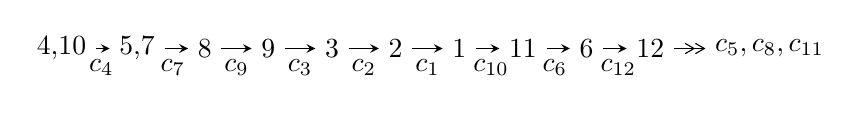
\begin{tikzpicture}[x=23pt, y=7pt]
	% node
	\node (A0) at (-1/8, 0) {4,10};
	\node (A1) at (17/16, 0) {5,7};
	\node (A2) at (17/8, 0) {8};
	\node (A3) at (25/8, 0) {9};
	\node (A4) at (33/8, 0) {3};
	\node (A5) at (41/8, 0) {2};
	\node (A6) at (49/8, 0) {1};
	\node (A7) at (57/8, 0) {11};
	\node (A8) at (65/8, 0) {6};
	\node (A9) at (73/8, 0) {12};
	\node (C1) at (1/2, -1) {$c_{4}$};
	\node (C2) at (13/8, -1) {$c_{7}$};
	\node (C3) at (21/8, -1) {$c_{9}$};
	\node (C4) at (29/8, -1) {$c_{3}$};
	\node (C5) at (37/8, -1) {$c_{2}$};
	\node (C6) at (45/8, -1) {$c_{1}$};
	\node (C7) at (53/8, -1) {$c_{10}$};
	\node (C8) at (61/8, -1) {$c_{6}$};
	\node (C9) at (69/8, -1) {$c_{12}$};
	\node (A10) at (11, 0) {$c_{5},c_{8},c_{11}$};

	% edge
	\draw[->,>=stealth]	
	(A0) edge (A1) (A1) edge (A2) (A2) edge (A3) (A3) edge (A4) (A4) edge (A5) (A5) edge (A6) (A6) edge (A7) (A7) edge (A8) (A8) edge (A9) ;
	\draw[->>,>={angle 60}]	
	(A9) edge (A10);
\end{tikzpicture} \\ 

\end{tabular} \\

\footnotetext{
The image of knot diagram is generated by the software ``\textbf{Draw programme}" developed by Andrew Bartholomew(\url{http://www.layer8.co.uk/maths/draw/index.htm\#Running-draw}), where we modified some parts for our purpose(\url{https://github.com/CATsTAILs/LinksPainter}).
}\phantom \\ \newline 
\centering \textbf{Ideals for irreducible components\footnotemark of $X_{\text{par}}$} 
 
\begin{align*}
I^u_{1}&=\langle 
8.98709\times10^{197} u^{57}+3.28099\times10^{198} u^{56}+\cdots+1.56771\times10^{200} b+3.12866\times10^{201},\\
\phantom{I^u_{1}}&\phantom{= \langle  }4.24469\times10^{201} u^{57}+9.55967\times10^{201} u^{56}+\cdots+1.61004\times10^{203} a+8.17316\times10^{204},\\
\phantom{I^u_{1}}&\phantom{= \langle  }u^{58}+u^{57}+\cdots+7117 u-1027\rangle \\
I^u_{2}&=\langle 
2.79079\times10^{21} u^{21}+1.76550\times10^{20} u^{20}+\cdots+2.38585\times10^{23} b-1.48787\times10^{23},\\
\phantom{I^u_{2}}&\phantom{= \langle  }4.29144\times10^{23} u^{21}+2.28509\times10^{23} u^{20}+\cdots+2.14726\times10^{24} a-1.05273\times10^{24},\;u^{22}-10 u^{20}+\cdots+73 u-9\rangle \\
\\
\end{align*}
\raggedright * 2 irreducible components of $\dim_{\mathbb{C}}=0$, with total 80 representations.\\
\footnotetext{All coefficients of polynomials are rational numbers. But the coefficients are sometimes approximated in decimal forms when there is not enough margin.}
\newpage
\renewcommand{\arraystretch}{1}
\centering \section*{I. $I^u_{1}= \langle 8.99\times10^{197} u^{57}+3.28\times10^{198} u^{56}+\cdots+1.57\times10^{200} b+3.13\times10^{201},\;4.24\times10^{201} u^{57}+9.56\times10^{201} u^{56}+\cdots+1.61\times10^{203} a+8.17\times10^{204},\;u^{58}+u^{57}+\cdots+7117 u-1027 \rangle$}
\flushleft \textbf{(i) Arc colorings}\\
\begin{tabular}{m{7pt} m{180pt} m{7pt} m{180pt} }
\flushright $a_{4}=$&$\begin{pmatrix}1\\0\end{pmatrix}$ \\
\flushright $a_{10}=$&$\begin{pmatrix}0\\u\end{pmatrix}$ \\
\flushright $a_{5}=$&$\begin{pmatrix}1\\u^2\end{pmatrix}$ \\
\flushright $a_{7}=$&$\begin{pmatrix}-0.0263639 u^{57}-0.0593753 u^{56}+\cdots+306.471 u-50.7637\\-0.00573262 u^{57}-0.0209285 u^{56}+\cdots+140.907 u-19.9569\end{pmatrix}$ \\
\flushright $a_{8}=$&$\begin{pmatrix}-0.0320965 u^{57}-0.0803038 u^{56}+\cdots+447.378 u-70.7206\\-0.00573262 u^{57}-0.0209285 u^{56}+\cdots+140.907 u-19.9569\end{pmatrix}$ \\
\flushright $a_{9}=$&$\begin{pmatrix}-0.0276476 u^{57}-0.0285016 u^{56}+\cdots-4.44141 u-21.8460\\-0.0133010 u^{57}-0.0190926 u^{56}+\cdots+17.6945 u-4.17250\end{pmatrix}$ \\
\flushright $a_{3}=$&$\begin{pmatrix}0.00962893 u^{57}+0.0347661 u^{56}+\cdots-153.709 u+17.1775\\0.00137276 u^{57}+0.0136626 u^{56}+\cdots-118.572 u+17.6094\end{pmatrix}$ \\
\flushright $a_{2}=$&$\begin{pmatrix}0.00962893 u^{57}+0.0347661 u^{56}+\cdots-153.709 u+17.1775\\-0.0130047 u^{57}-0.0227497 u^{56}+\cdots+50.4397 u-8.20641\end{pmatrix}$ \\
\flushright $a_{1}=$&$\begin{pmatrix}-0.00337579 u^{57}+0.0120164 u^{56}+\cdots-103.269 u+8.97114\\-0.0130047 u^{57}-0.0227497 u^{56}+\cdots+50.4397 u-8.20641\end{pmatrix}$ \\
\flushright $a_{11}=$&$\begin{pmatrix}0.0273854 u^{57}+0.0503706 u^{56}+\cdots-200.581 u+48.9873\\0.0113327 u^{57}+0.0369171 u^{56}+\cdots-227.216 u+32.7951\end{pmatrix}$ \\
\flushright $a_{6}=$&$\begin{pmatrix}-0.00894778 u^{57}-0.00254877 u^{56}+\cdots-150.638 u+30.0737\\0.0204778 u^{57}+0.0335185 u^{56}+\cdots-83.8092 u+15.3951\end{pmatrix}$ \\
\flushright $a_{12}=$&$\begin{pmatrix}-0.0314997 u^{57}-0.0527340 u^{56}+\cdots+69.4621 u-13.0531\\-0.0300231 u^{57}-0.0787118 u^{56}+\cdots+398.575 u-61.1428\end{pmatrix}$\\&\end{tabular}
\flushleft \textbf{(ii) Obstruction class $= -1$}\\~\\
\flushleft \textbf{(iii) Cusp Shapes $= -0.0373141 u^{57}-0.119218 u^{56}+\cdots+753.945 u-118.284$}\\~\\
\newpage\renewcommand{\arraystretch}{1}
\flushleft \textbf{(iv) u-Polynomials at the component}\newline \\
\begin{tabular}{m{50pt}|m{274pt}}
Crossings & \hspace{64pt}u-Polynomials at each crossing \\
\hline $$\begin{aligned}c_{1}\end{aligned}$$&$\begin{aligned}
&u^{58}+7 u^{57}+\cdots-22459 u+1219
\end{aligned}$\\
\hline $$\begin{aligned}c_{2}\end{aligned}$$&$\begin{aligned}
&u^{58}+4 u^{57}+\cdots+1084 u+167
\end{aligned}$\\
\hline $$\begin{aligned}c_{3}\end{aligned}$$&$\begin{aligned}
&u^{58}+u^{57}+\cdots-283 u-43
\end{aligned}$\\
\hline $$\begin{aligned}c_{4}\end{aligned}$$&$\begin{aligned}
&u^{58}- u^{57}+\cdots-7117 u-1027
\end{aligned}$\\
\hline $$\begin{aligned}c_{5},c_{12}\end{aligned}$$&$\begin{aligned}
&u^{58}+2 u^{57}+\cdots+1960 u+664
\end{aligned}$\\
\hline $$\begin{aligned}c_{6}\end{aligned}$$&$\begin{aligned}
&u^{58}+6 u^{57}+\cdots+10 u+1
\end{aligned}$\\
\hline $$\begin{aligned}c_{7}\end{aligned}$$&$\begin{aligned}
&u^{58}+9 u^{56}+\cdots-10008 u-584
\end{aligned}$\\
\hline $$\begin{aligned}c_{8},c_{11}\end{aligned}$$&$\begin{aligned}
&u^{58}+u^{57}+\cdots+1066 u+97
\end{aligned}$\\
\hline $$\begin{aligned}c_{9}\end{aligned}$$&$\begin{aligned}
&u^{58}+u^{57}+\cdots+u-1
\end{aligned}$\\
\hline $$\begin{aligned}c_{10}\end{aligned}$$&$\begin{aligned}
&u^{58}-4 u^{57}+\cdots+129032 u-9829
\end{aligned}$\\
\hline
\end{tabular}\\~\\
\newpage\renewcommand{\arraystretch}{1}
\flushleft \textbf{(v) Riley Polynomials at the component}\newline \\
\begin{tabular}{m{50pt}|m{274pt}}
Crossings & \hspace{64pt}Riley Polynomials at each crossing \\
\hline $$\begin{aligned}c_{1}\end{aligned}$$&$\begin{aligned}
&y^{58}-61 y^{57}+\cdots-240710163 y+1485961
\end{aligned}$\\
\hline $$\begin{aligned}c_{2}\end{aligned}$$&$\begin{aligned}
&y^{58}-8 y^{57}+\cdots-98574 y+27889
\end{aligned}$\\
\hline $$\begin{aligned}c_{3}\end{aligned}$$&$\begin{aligned}
&y^{58}-9 y^{57}+\cdots-167293 y+1849
\end{aligned}$\\
\hline $$\begin{aligned}c_{4}\end{aligned}$$&$\begin{aligned}
&y^{58}-67 y^{57}+\cdots-53586855 y+1054729
\end{aligned}$\\
\hline $$\begin{aligned}c_{5},c_{12}\end{aligned}$$&$\begin{aligned}
&y^{58}+36 y^{57}+\cdots-6938496 y+440896
\end{aligned}$\\
\hline $$\begin{aligned}c_{6}\end{aligned}$$&$\begin{aligned}
&y^{58}+8 y^{57}+\cdots-184 y+1
\end{aligned}$\\
\hline $$\begin{aligned}c_{7}\end{aligned}$$&$\begin{aligned}
&y^{58}+18 y^{57}+\cdots-5014784 y+341056
\end{aligned}$\\
\hline $$\begin{aligned}c_{8},c_{11}\end{aligned}$$&$\begin{aligned}
&y^{58}+23 y^{57}+\cdots+106020 y+9409
\end{aligned}$\\
\hline $$\begin{aligned}c_{9}\end{aligned}$$&$\begin{aligned}
&y^{58}-19 y^{57}+\cdots-27 y+1
\end{aligned}$\\
\hline $$\begin{aligned}c_{10}\end{aligned}$$&$\begin{aligned}
&y^{58}-52 y^{57}+\cdots-2754353568 y+96609241
\end{aligned}$\\
\hline
\end{tabular}\\~\\
\newpage\flushleft \textbf{(vi) Complex Volumes and Cusp Shapes}
$$\begin{array}{c|c|c}  
\text{Solutions to }I^u_{1}& \I (\text{vol} + \sqrt{-1}CS) & \text{Cusp shape}\\
 \hline 
\begin{aligned}
u &= -0.984047 + 0.106547 I \\
a &= \phantom{-}0.732984 + 0.485124 I \\
b &= -0.71312 + 2.03208 I\end{aligned}
 & -5.10938 - 4.31500 I & \phantom{-0.000000 } 0 \\ \hline\begin{aligned}
u &= -0.984047 - 0.106547 I \\
a &= \phantom{-}0.732984 - 0.485124 I \\
b &= -0.71312 - 2.03208 I\end{aligned}
 & -5.10938 + 4.31500 I & \phantom{-0.000000 } 0 \\ \hline\begin{aligned}
u &= \phantom{-}0.951459 + 0.036280 I \\
a &= \phantom{-}0.756616 + 0.985473 I \\
b &= -0.14380 + 1.51989 I\end{aligned}
 & \phantom{-}2.83534 - 4.32094 I & \phantom{-0.000000 } 0 \\ \hline\begin{aligned}
u &= \phantom{-}0.951459 - 0.036280 I \\
a &= \phantom{-}0.756616 - 0.985473 I \\
b &= -0.14380 - 1.51989 I\end{aligned}
 & \phantom{-}2.83534 + 4.32094 I & \phantom{-0.000000 } 0 \\ \hline\begin{aligned}
u &= \phantom{-}0.889685 + 0.338008 I \\
a &= \phantom{-}1.06446 - 1.48155 I \\
b &= -0.428769 - 0.679768 I\end{aligned}
 & -0.25157 + 3.22294 I & \phantom{-0.000000 } 0 \\ \hline\begin{aligned}
u &= \phantom{-}0.889685 - 0.338008 I \\
a &= \phantom{-}1.06446 + 1.48155 I \\
b &= -0.428769 + 0.679768 I\end{aligned}
 & -0.25157 - 3.22294 I & \phantom{-0.000000 } 0 \\ \hline\begin{aligned}
u &= \phantom{-}0.938379 + 0.011522 I \\
a &= -0.161328 - 0.401628 I \\
b &= \phantom{-}0.308280 + 0.060433 I\end{aligned}
 & -1.102690 - 0.062220 I & \phantom{-0.000000 } 0 \\ \hline\begin{aligned}
u &= \phantom{-}0.938379 - 0.011522 I \\
a &= -0.161328 + 0.401628 I \\
b &= \phantom{-}0.308280 - 0.060433 I\end{aligned}
 & -1.102690 + 0.062220 I & \phantom{-0.000000 } 0 \\ \hline\begin{aligned}
u &= -0.735401 + 0.007028 I \\
a &= \phantom{-}1.37029 - 1.13833 I \\
b &= -0.71739 - 1.26490 I\end{aligned}
 & \phantom{-}4.02435 + 6.74078 I & -6.40897 - 6.18806 I \\ \hline\begin{aligned}
u &= -0.735401 - 0.007028 I \\
a &= \phantom{-}1.37029 + 1.13833 I \\
b &= -0.71739 + 1.26490 I\end{aligned}
 & \phantom{-}4.02435 - 6.74078 I & -6.40897 + 6.18806 I\\
 \hline 
 \end{array}$$\newpage$$\begin{array}{c|c|c}  
\text{Solutions to }I^u_{1}& \I (\text{vol} + \sqrt{-1}CS) & \text{Cusp shape}\\
 \hline 
\begin{aligned}
u &= \phantom{-}0.611627 + 0.386837 I \\
a &= \phantom{-}1.49854 - 0.36748 I \\
b &= -0.269457 + 0.990833 I\end{aligned}
 & \phantom{-}0.571664 - 1.277470 I & -8.81085 + 0.40906 I \\ \hline\begin{aligned}
u &= \phantom{-}0.611627 - 0.386837 I \\
a &= \phantom{-}1.49854 + 0.36748 I \\
b &= -0.269457 - 0.990833 I\end{aligned}
 & \phantom{-}0.571664 + 1.277470 I & -8.81085 - 0.40906 I \\ \hline\begin{aligned}
u &= -0.543172 + 0.422725 I \\
a &= \phantom{-}0.719118 + 0.935767 I \\
b &= -1.320790 + 0.324187 I\end{aligned}
 & \phantom{-}4.86373 + 2.09347 I & -6.47153 - 2.48732 I \\ \hline\begin{aligned}
u &= -0.543172 - 0.422725 I \\
a &= \phantom{-}0.719118 - 0.935767 I \\
b &= -1.320790 - 0.324187 I\end{aligned}
 & \phantom{-}4.86373 - 2.09347 I & -6.47153 + 2.48732 I \\ \hline\begin{aligned}
u &= \phantom{-}1.208100 + 0.579060 I \\
a &= -0.037426 - 0.757251 I \\
b &= \phantom{-}0.521975 - 0.291948 I\end{aligned}
 & -0.975445 - 0.218387 I & \phantom{-0.000000 } 0 \\ \hline\begin{aligned}
u &= \phantom{-}1.208100 - 0.579060 I \\
a &= -0.037426 + 0.757251 I \\
b &= \phantom{-}0.521975 + 0.291948 I\end{aligned}
 & -0.975445 + 0.218387 I & \phantom{-0.000000 } 0 \\ \hline\begin{aligned}
u &= \phantom{-}0.660076\phantom{ +0.000000I} \\
a &= \phantom{-}0.366125\phantom{ +0.000000I} \\
b &= \phantom{-}0.323077\phantom{ +0.000000I}\end{aligned}
 & -1.09302\phantom{ +0.000000I} & -7.08600\phantom{ +0.000000I} \\ \hline\begin{aligned}
u &= -0.554976 + 0.140362 I \\
a &= \phantom{-}1.75463 - 1.19601 I \\
b &= \phantom{-}0.273584 + 0.107138 I\end{aligned}
 & \phantom{-}4.60137 - 0.26241 I & -5.57820 + 1.37492 I \\ \hline\begin{aligned}
u &= -0.554976 - 0.140362 I \\
a &= \phantom{-}1.75463 + 1.19601 I \\
b &= \phantom{-}0.273584 - 0.107138 I\end{aligned}
 & \phantom{-}4.60137 + 0.26241 I & -5.57820 - 1.37492 I \\ \hline\begin{aligned}
u &= \phantom{-}1.34287 + 0.51625 I \\
a &= \phantom{-}0.360673 - 0.444881 I \\
b &= -0.86318 - 2.71719 I\end{aligned}
 & -1.29465 - 2.40549 I & \phantom{-0.000000 } 0\\
 \hline 
 \end{array}$$\newpage$$\begin{array}{c|c|c}  
\text{Solutions to }I^u_{1}& \I (\text{vol} + \sqrt{-1}CS) & \text{Cusp shape}\\
 \hline 
\begin{aligned}
u &= \phantom{-}1.34287 - 0.51625 I \\
a &= \phantom{-}0.360673 + 0.444881 I \\
b &= -0.86318 + 2.71719 I\end{aligned}
 & -1.29465 + 2.40549 I & \phantom{-0.000000 } 0 \\ \hline\begin{aligned}
u &= -1.09636 + 0.94746 I \\
a &= \phantom{-}0.401125 + 0.121349 I \\
b &= \phantom{-}0.133549 - 1.228370 I\end{aligned}
 & -4.43749 - 1.69406 I & \phantom{-0.000000 } 0 \\ \hline\begin{aligned}
u &= -1.09636 - 0.94746 I \\
a &= \phantom{-}0.401125 - 0.121349 I \\
b &= \phantom{-}0.133549 + 1.228370 I\end{aligned}
 & -4.43749 + 1.69406 I & \phantom{-0.000000 } 0 \\ \hline\begin{aligned}
u &= -0.479931 + 0.256201 I \\
a &= \phantom{-}0.80829 + 1.69787 I \\
b &= \phantom{-}0.357974 - 0.899794 I\end{aligned}
 & \phantom{-}4.89868 - 5.92269 I & -8.28735 + 6.67085 I \\ \hline\begin{aligned}
u &= -0.479931 - 0.256201 I \\
a &= \phantom{-}0.80829 - 1.69787 I \\
b &= \phantom{-}0.357974 + 0.899794 I\end{aligned}
 & \phantom{-}4.89868 + 5.92269 I & -8.28735 - 6.67085 I \\ \hline\begin{aligned}
u &= -1.45716\phantom{ +0.000000I} \\
a &= -0.652587\phantom{ +0.000000I} \\
b &= \phantom{-}1.66458\phantom{ +0.000000I}\end{aligned}
 & -6.65741\phantom{ +0.000000I} & \phantom{-0.000000 } 0 \\ \hline\begin{aligned}
u &= \phantom{-}1.51660 + 0.17170 I \\
a &= -0.397509 - 0.123089 I \\
b &= \phantom{-}2.78994 - 1.29874 I\end{aligned}
 & -2.05878 - 4.62210 I & \phantom{-0.000000 } 0 \\ \hline\begin{aligned}
u &= \phantom{-}1.51660 - 0.17170 I \\
a &= -0.397509 + 0.123089 I \\
b &= \phantom{-}2.78994 + 1.29874 I\end{aligned}
 & -2.05878 + 4.62210 I & \phantom{-0.000000 } 0 \\ \hline\begin{aligned}
u &= \phantom{-}0.159997 + 0.444223 I \\
a &= -0.891005 - 0.942470 I \\
b &= -0.215135 + 1.292810 I\end{aligned}
 & \phantom{-}5.40486 + 3.03261 I & -1.43535 + 3.06435 I \\ \hline\begin{aligned}
u &= \phantom{-}0.159997 - 0.444223 I \\
a &= -0.891005 + 0.942470 I \\
b &= -0.215135 - 1.292810 I\end{aligned}
 & \phantom{-}5.40486 - 3.03261 I & -1.43535 - 3.06435 I\\
 \hline 
 \end{array}$$\newpage$$\begin{array}{c|c|c}  
\text{Solutions to }I^u_{1}& \I (\text{vol} + \sqrt{-1}CS) & \text{Cusp shape}\\
 \hline 
\begin{aligned}
u &= -1.55519 + 0.00032 I \\
a &= -0.587461 - 0.437982 I \\
b &= \phantom{-}0.67801 - 1.40728 I\end{aligned}
 & -6.26258 - 2.81974 I & \phantom{-0.000000 } 0 \\ \hline\begin{aligned}
u &= -1.55519 - 0.00032 I \\
a &= -0.587461 + 0.437982 I \\
b &= \phantom{-}0.67801 + 1.40728 I\end{aligned}
 & -6.26258 + 2.81974 I & \phantom{-0.000000 } 0 \\ \hline\begin{aligned}
u &= \phantom{-}0.127053 + 0.418851 I \\
a &= \phantom{-}1.23833 - 1.01400 I \\
b &= -0.126610 + 0.836327 I\end{aligned}
 & -0.617637 - 1.214780 I & -6.10791 + 5.67942 I \\ \hline\begin{aligned}
u &= \phantom{-}0.127053 - 0.418851 I \\
a &= \phantom{-}1.23833 + 1.01400 I \\
b &= -0.126610 - 0.836327 I\end{aligned}
 & -0.617637 + 1.214780 I & -6.10791 - 5.67942 I \\ \hline\begin{aligned}
u &= -1.63145\phantom{ +0.000000I} \\
a &= \phantom{-}0.436826\phantom{ +0.000000I} \\
b &= -1.65196\phantom{ +0.000000I}\end{aligned}
 & -9.90939\phantom{ +0.000000I} & \phantom{-0.000000 } 0 \\ \hline\begin{aligned}
u &= \phantom{-}1.76333 + 0.03132 I \\
a &= -0.750182 + 0.469345 I \\
b &= \phantom{-}1.20433 + 1.24812 I\end{aligned}
 & -4.94459 + 6.18934 I & \phantom{-0.000000 } 0 \\ \hline\begin{aligned}
u &= \phantom{-}1.76333 - 0.03132 I \\
a &= -0.750182 - 0.469345 I \\
b &= \phantom{-}1.20433 - 1.24812 I\end{aligned}
 & -4.94459 - 6.18934 I & \phantom{-0.000000 } 0 \\ \hline\begin{aligned}
u &= \phantom{-}0.222347 + 0.057423 I \\
a &= \phantom{-}4.52994 + 3.59770 I \\
b &= -0.062776 - 0.383104 I\end{aligned}
 & \phantom{-}1.83627 - 4.60135 I & -3.06433 + 1.23782 I \\ \hline\begin{aligned}
u &= \phantom{-}0.222347 - 0.057423 I \\
a &= \phantom{-}4.52994 - 3.59770 I \\
b &= -0.062776 + 0.383104 I\end{aligned}
 & \phantom{-}1.83627 + 4.60135 I & -3.06433 - 1.23782 I \\ \hline\begin{aligned}
u &= -0.48982 + 1.70817 I \\
a &= \phantom{-}0.647515 + 0.422020 I \\
b &= -1.71821 + 0.15561 I\end{aligned}
 & \phantom{-}6.18677 + 0.35665 I & \phantom{-0.000000 } 0\\
 \hline 
 \end{array}$$\newpage$$\begin{array}{c|c|c}  
\text{Solutions to }I^u_{1}& \I (\text{vol} + \sqrt{-1}CS) & \text{Cusp shape}\\
 \hline 
\begin{aligned}
u &= -0.48982 - 1.70817 I \\
a &= \phantom{-}0.647515 - 0.422020 I \\
b &= -1.71821 - 0.15561 I\end{aligned}
 & \phantom{-}6.18677 - 0.35665 I & \phantom{-0.000000 } 0 \\ \hline\begin{aligned}
u &= -1.79356 + 0.11460 I \\
a &= -0.715949 + 0.568710 I \\
b &= \phantom{-}0.49033 + 1.44237 I\end{aligned}
 & -7.85182 + 4.36860 I & \phantom{-0.000000 } 0 \\ \hline\begin{aligned}
u &= -1.79356 - 0.11460 I \\
a &= -0.715949 - 0.568710 I \\
b &= \phantom{-}0.49033 - 1.44237 I\end{aligned}
 & -7.85182 - 4.36860 I & \phantom{-0.000000 } 0 \\ \hline\begin{aligned}
u &= \phantom{-}1.62131 + 0.77787 I \\
a &= \phantom{-}0.785352 + 0.143559 I \\
b &= -1.54041 + 1.26825 I\end{aligned}
 & -2.94636 - 6.95100 I & \phantom{-0.000000 } 0 \\ \hline\begin{aligned}
u &= \phantom{-}1.62131 - 0.77787 I \\
a &= \phantom{-}0.785352 - 0.143559 I \\
b &= -1.54041 - 1.26825 I\end{aligned}
 & -2.94636 + 6.95100 I & \phantom{-0.000000 } 0 \\ \hline\begin{aligned}
u &= -1.75534 + 0.48896 I \\
a &= \phantom{-}0.227519 + 0.805258 I \\
b &= \phantom{-}0.410897 + 0.818197 I\end{aligned}
 & \phantom{-}0.70429 + 7.95243 I & \phantom{-0.000000 } 0 \\ \hline\begin{aligned}
u &= -1.75534 - 0.48896 I \\
a &= \phantom{-}0.227519 - 0.805258 I \\
b &= \phantom{-}0.410897 - 0.818197 I\end{aligned}
 & \phantom{-}0.70429 - 7.95243 I & \phantom{-0.000000 } 0 \\ \hline\begin{aligned}
u &= -1.80778 + 0.38348 I \\
a &= -0.171765 - 0.343297 I \\
b &= \phantom{-}0.191963 - 0.552646 I\end{aligned}
 & -3.74606 - 2.72375 I & \phantom{-0.000000 } 0 \\ \hline\begin{aligned}
u &= -1.80778 - 0.38348 I \\
a &= -0.171765 + 0.343297 I \\
b &= \phantom{-}0.191963 + 0.552646 I\end{aligned}
 & -3.74606 + 2.72375 I & \phantom{-0.000000 } 0 \\ \hline\begin{aligned}
u &= \phantom{-}1.90742 + 0.23418 I \\
a &= -0.392220 - 0.010291 I \\
b &= -0.096402 - 0.583283 I\end{aligned}
 & -2.82054 + 3.11371 I & \phantom{-0.000000 } 0\\
 \hline 
 \end{array}$$\newpage$$\begin{array}{c|c|c}  
\text{Solutions to }I^u_{1}& \I (\text{vol} + \sqrt{-1}CS) & \text{Cusp shape}\\
 \hline 
\begin{aligned}
u &= \phantom{-}1.90742 - 0.23418 I \\
a &= -0.392220 + 0.010291 I \\
b &= -0.096402 + 0.583283 I\end{aligned}
 & -2.82054 - 3.11371 I & \phantom{-0.000000 } 0 \\ \hline\begin{aligned}
u &= -1.87242 + 0.53585 I \\
a &= \phantom{-}0.710787 - 0.294332 I \\
b &= -1.36569 - 1.62804 I\end{aligned}
 & -0.6525 + 15.7491 I & \phantom{-0.000000 } 0 \\ \hline\begin{aligned}
u &= -1.87242 - 0.53585 I \\
a &= \phantom{-}0.710787 + 0.294332 I \\
b &= -1.36569 + 1.62804 I\end{aligned}
 & -0.6525 - 15.7491 I & \phantom{-0.000000 } 0 \\ \hline\begin{aligned}
u &= -1.96832\phantom{ +0.000000I} \\
a &= -1.31909\phantom{ +0.000000I} \\
b &= \phantom{-}0.902042\phantom{ +0.000000I}\end{aligned}
 & -11.0216\phantom{ +0.000000I} & \phantom{-0.000000 } 0 \\ \hline\begin{aligned}
u &= \phantom{-}0.12762 + 2.16706 I \\
a &= -0.451547 + 0.382090 I \\
b &= \phantom{-}1.61400 - 0.44696 I\end{aligned}
 & \phantom{-}6.61103 - 6.39087 I & \phantom{-0.000000 } 0 \\ \hline\begin{aligned}
u &= \phantom{-}0.12762 - 2.16706 I \\
a &= -0.451547 - 0.382090 I \\
b &= \phantom{-}1.61400 + 0.44696 I\end{aligned}
 & \phantom{-}6.61103 + 6.39087 I & \phantom{-0.000000 } 0 \\ \hline\begin{aligned}
u &= \phantom{-}1.97864 + 0.91027 I \\
a &= \phantom{-}0.389495 + 0.063606 I \\
b &= -0.011945 + 1.259660 I\end{aligned}
 & -1.21978 - 5.87932 I & \phantom{-0.000000 } 0 \\ \hline\begin{aligned}
u &= \phantom{-}1.97864 - 0.91027 I \\
a &= \phantom{-}0.389495 - 0.063606 I \\
b &= -0.011945 - 1.259660 I\end{aligned}
 & -1.21978 + 5.87932 I & \phantom{-0.000000 } 0\\
 \hline 
 \end{array}$$\newpage\newpage\renewcommand{\arraystretch}{1}
\centering \section*{II. $I^u_{2}= \langle 2.79\times10^{21} u^{21}+1.77\times10^{20} u^{20}+\cdots+2.39\times10^{23} b-1.49\times10^{23},\;4.29\times10^{23} u^{21}+2.29\times10^{23} u^{20}+\cdots+2.15\times10^{24} a-1.05\times10^{24},\;u^{22}-10 u^{20}+\cdots+73 u-9 \rangle$}
\flushleft \textbf{(i) Arc colorings}\\
\begin{tabular}{m{7pt} m{180pt} m{7pt} m{180pt} }
\flushright $a_{4}=$&$\begin{pmatrix}1\\0\end{pmatrix}$ \\
\flushright $a_{10}=$&$\begin{pmatrix}0\\u\end{pmatrix}$ \\
\flushright $a_{5}=$&$\begin{pmatrix}1\\u^2\end{pmatrix}$ \\
\flushright $a_{7}=$&$\begin{pmatrix}-0.199856 u^{21}-0.106419 u^{20}+\cdots+19.6045 u+0.490264\\-0.0116973 u^{21}-0.000739990 u^{20}+\cdots-7.08742 u+0.623622\end{pmatrix}$ \\
\flushright $a_{8}=$&$\begin{pmatrix}-0.211553 u^{21}-0.107159 u^{20}+\cdots+12.5171 u+1.11389\\-0.0116973 u^{21}-0.000739990 u^{20}+\cdots-7.08742 u+0.623622\end{pmatrix}$ \\
\flushright $a_{9}=$&$\begin{pmatrix}-0.336127 u^{21}-0.0767089 u^{20}+\cdots+51.7425 u-6.09472\\-0.00505495 u^{21}+0.0250633 u^{20}+\cdots-1.05021 u+0.800312\end{pmatrix}$ \\
\flushright $a_{3}=$&$\begin{pmatrix}0.324297 u^{21}+0.300057 u^{20}+\cdots-20.7701 u+6.75595\\0.179573 u^{21}+0.111102 u^{20}+\cdots-23.5518 u+3.45052\end{pmatrix}$ \\
\flushright $a_{2}=$&$\begin{pmatrix}0.324297 u^{21}+0.300057 u^{20}+\cdots-20.7701 u+6.75595\\-0.0962234 u^{21}-0.138807 u^{20}+\cdots-4.56630 u+0.750012\end{pmatrix}$ \\
\flushright $a_{1}=$&$\begin{pmatrix}0.228074 u^{21}+0.161250 u^{20}+\cdots-25.3364 u+7.50597\\-0.0962234 u^{21}-0.138807 u^{20}+\cdots-4.56630 u+0.750012\end{pmatrix}$ \\
\flushright $a_{11}=$&$\begin{pmatrix}0.318413 u^{21}+0.152269 u^{20}+\cdots-39.8613 u+2.56934\\-0.0745587 u^{21}-0.0585677 u^{20}+\cdots+12.8859 u-2.38557\end{pmatrix}$ \\
\flushright $a_{6}=$&$\begin{pmatrix}0.417332 u^{21}+0.134515 u^{20}+\cdots-84.2017 u+11.3295\\0.0872425 u^{21}+0.0721007 u^{20}+\cdots-7.96511 u-0.936957\end{pmatrix}$ \\
\flushright $a_{12}=$&$\begin{pmatrix}-0.196498 u^{21}-0.237839 u^{20}+\cdots+11.6692 u-7.14808\\-0.238971 u^{21}-0.175726 u^{20}+\cdots+32.6164 u-4.66605\end{pmatrix}$\\&\end{tabular}
\flushleft \textbf{(ii) Obstruction class $= 1$}\\~\\
\flushleft \textbf{(iii) Cusp Shapes $= -\frac{457412961431615476330833}{238584851591663803618957} u^{21}-\frac{254429452136571387242067}{238584851591663803618957} u^{20}+\cdots+\frac{58966595376988644279933534}{238584851591663803618957} u-\frac{10233901156098748389216510}{238584851591663803618957}$}\\~\\
\newpage\renewcommand{\arraystretch}{1}
\flushleft \textbf{(iv) u-Polynomials at the component}\newline \\
\begin{tabular}{m{50pt}|m{274pt}}
Crossings & \hspace{64pt}u-Polynomials at each crossing \\
\hline $$\begin{aligned}c_{1}\end{aligned}$$&$\begin{aligned}
&u^{22}-12 u^{21}+\cdots-9 u+1
\end{aligned}$\\
\hline $$\begin{aligned}c_{2}\end{aligned}$$&$\begin{aligned}
&u^{22}- u^{21}+\cdots+72 u-63
\end{aligned}$\\
\hline $$\begin{aligned}c_{3}\end{aligned}$$&$\begin{aligned}
&u^{22}- u^{20}+\cdots-7 u+1
\end{aligned}$\\
\hline $$\begin{aligned}c_{4}\end{aligned}$$&$\begin{aligned}
&u^{22}-10 u^{20}+\cdots+73 u-9
\end{aligned}$\\
\hline $$\begin{aligned}c_{5}\end{aligned}$$&$\begin{aligned}
&u^{22}- u^{21}+\cdots+24 u+8
\end{aligned}$\\
\hline $$\begin{aligned}c_{6}\end{aligned}$$&$\begin{aligned}
&u^{22}- u^{21}+\cdots-16 u-3
\end{aligned}$\\
\hline $$\begin{aligned}c_{7}\end{aligned}$$&$\begin{aligned}
&u^{22}+3 u^{21}+\cdots+8 u-56
\end{aligned}$\\
\hline $$\begin{aligned}c_{8}\end{aligned}$$&$\begin{aligned}
&u^{22}-2 u^{21}+\cdots+2 u+1
\end{aligned}$\\
\hline $$\begin{aligned}c_{9}\end{aligned}$$&$\begin{aligned}
&u^{22}+6 u^{21}+\cdots+5 u+1
\end{aligned}$\\
\hline $$\begin{aligned}c_{10}\end{aligned}$$&$\begin{aligned}
&u^{22}-7 u^{21}+\cdots+20 u-7
\end{aligned}$\\
\hline $$\begin{aligned}c_{11}\end{aligned}$$&$\begin{aligned}
&u^{22}+2 u^{21}+\cdots-2 u+1
\end{aligned}$\\
\hline $$\begin{aligned}c_{12}\end{aligned}$$&$\begin{aligned}
&u^{22}+u^{21}+\cdots-24 u+8
\end{aligned}$\\
\hline
\end{tabular}\\~\\
\newpage\renewcommand{\arraystretch}{1}
\flushleft \textbf{(v) Riley Polynomials at the component}\newline \\
\begin{tabular}{m{50pt}|m{274pt}}
Crossings & \hspace{64pt}Riley Polynomials at each crossing \\
\hline $$\begin{aligned}c_{1}\end{aligned}$$&$\begin{aligned}
&y^{22}-22 y^{21}+\cdots+83 y+1
\end{aligned}$\\
\hline $$\begin{aligned}c_{2}\end{aligned}$$&$\begin{aligned}
&y^{22}-13 y^{21}+\cdots-12240 y+3969
\end{aligned}$\\
\hline $$\begin{aligned}c_{3}\end{aligned}$$&$\begin{aligned}
&y^{22}-2 y^{21}+\cdots-31 y+1
\end{aligned}$\\
\hline $$\begin{aligned}c_{4}\end{aligned}$$&$\begin{aligned}
&y^{22}-20 y^{21}+\cdots+395 y+81
\end{aligned}$\\
\hline $$\begin{aligned}c_{5},c_{12}\end{aligned}$$&$\begin{aligned}
&y^{22}+7 y^{21}+\cdots+64 y+64
\end{aligned}$\\
\hline $$\begin{aligned}c_{6}\end{aligned}$$&$\begin{aligned}
&y^{22}-5 y^{21}+\cdots-34 y+9
\end{aligned}$\\
\hline $$\begin{aligned}c_{7}\end{aligned}$$&$\begin{aligned}
&y^{22}+5 y^{21}+\cdots+39360 y+3136
\end{aligned}$\\
\hline $$\begin{aligned}c_{8},c_{11}\end{aligned}$$&$\begin{aligned}
&y^{22}+6 y^{21}+\cdots-2 y+1
\end{aligned}$\\
\hline $$\begin{aligned}c_{9}\end{aligned}$$&$\begin{aligned}
&y^{22}-12 y^{21}+\cdots-13 y+1
\end{aligned}$\\
\hline $$\begin{aligned}c_{10}\end{aligned}$$&$\begin{aligned}
&y^{22}-21 y^{21}+\cdots+6 y+49
\end{aligned}$\\
\hline
\end{tabular}\\~\\
\newpage\flushleft \textbf{(vi) Complex Volumes and Cusp Shapes}
$$\begin{array}{c|c|c}  
\text{Solutions to }I^u_{2}& \I (\text{vol} + \sqrt{-1}CS) & \text{Cusp shape}\\
 \hline 
\begin{aligned}
u &= \phantom{-}1.074930 + 0.105891 I \\
a &= \phantom{-}1.065490 - 0.834834 I \\
b &= -0.116473 - 0.664580 I\end{aligned}
 & -0.49759 + 2.56520 I & -11.45169 - 0.03293 I \\ \hline\begin{aligned}
u &= \phantom{-}1.074930 - 0.105891 I \\
a &= \phantom{-}1.065490 + 0.834834 I \\
b &= -0.116473 + 0.664580 I\end{aligned}
 & -0.49759 - 2.56520 I & -11.45169 + 0.03293 I \\ \hline\begin{aligned}
u &= -0.534288 + 0.431482 I \\
a &= -0.434617 - 1.025970 I \\
b &= -0.157192 + 0.475540 I\end{aligned}
 & -1.81004 - 0.52019 I & -15.0020 + 3.2051 I \\ \hline\begin{aligned}
u &= -0.534288 - 0.431482 I \\
a &= -0.434617 + 1.025970 I \\
b &= -0.157192 - 0.475540 I\end{aligned}
 & -1.81004 + 0.52019 I & -15.0020 - 3.2051 I \\ \hline\begin{aligned}
u &= \phantom{-}0.661139 + 0.110313 I \\
a &= \phantom{-}1.56420 + 1.41244 I \\
b &= -0.229898 + 0.895312 I\end{aligned}
 & \phantom{-}1.36966 - 5.12657 I & -11.4526 + 9.5918 I \\ \hline\begin{aligned}
u &= \phantom{-}0.661139 - 0.110313 I \\
a &= \phantom{-}1.56420 - 1.41244 I \\
b &= -0.229898 - 0.895312 I\end{aligned}
 & \phantom{-}1.36966 + 5.12657 I & -11.4526 - 9.5918 I \\ \hline\begin{aligned}
u &= \phantom{-}1.395400 + 0.151449 I \\
a &= -0.635171 + 0.368343 I \\
b &= \phantom{-}1.07115 + 1.63083 I\end{aligned}
 & -6.51584 + 4.02828 I & -15.4736 - 6.2870 I \\ \hline\begin{aligned}
u &= \phantom{-}1.395400 - 0.151449 I \\
a &= -0.635171 - 0.368343 I \\
b &= \phantom{-}1.07115 - 1.63083 I\end{aligned}
 & -6.51584 - 4.02828 I & -15.4736 + 6.2870 I \\ \hline\begin{aligned}
u &= -0.51433 + 1.35727 I \\
a &= \phantom{-}0.844430 + 0.510048 I \\
b &= -1.50481 + 0.10273 I\end{aligned}
 & \phantom{-}6.84628 + 0.34484 I & \phantom{-}0.584936 + 0.037274 I \\ \hline\begin{aligned}
u &= -0.51433 - 1.35727 I \\
a &= \phantom{-}0.844430 - 0.510048 I \\
b &= -1.50481 - 0.10273 I\end{aligned}
 & \phantom{-}6.84628 - 0.34484 I & \phantom{-}0.584936 - 0.037274 I\\
 \hline 
 \end{array}$$\newpage$$\begin{array}{c|c|c}  
\text{Solutions to }I^u_{2}& \I (\text{vol} + \sqrt{-1}CS) & \text{Cusp shape}\\
 \hline 
\begin{aligned}
u &= \phantom{-}0.07066 + 1.58496 I \\
a &= -0.581666 + 0.511900 I \\
b &= \phantom{-}1.29498 - 0.63093 I\end{aligned}
 & \phantom{-}7.58470 - 6.19359 I & -1.94969 + 4.30160 I \\ \hline\begin{aligned}
u &= \phantom{-}0.07066 - 1.58496 I \\
a &= -0.581666 - 0.511900 I \\
b &= \phantom{-}1.29498 + 0.63093 I\end{aligned}
 & \phantom{-}7.58470 + 6.19359 I & -1.94969 - 4.30160 I \\ \hline\begin{aligned}
u &= \phantom{-}1.62037\phantom{ +0.000000I} \\
a &= \phantom{-}0.458428\phantom{ +0.000000I} \\
b &= -1.67473\phantom{ +0.000000I}\end{aligned}
 & -9.98265\phantom{ +0.000000I} & -65.6220\phantom{ +0.000000I} \\ \hline\begin{aligned}
u &= \phantom{-}1.38984 + 0.85119 I \\
a &= -0.299446 + 0.142790 I \\
b &= \phantom{-}0.092686 - 1.119880 I\end{aligned}
 & -4.73458 + 2.11091 I & -18.7205 - 5.4471 I \\ \hline\begin{aligned}
u &= \phantom{-}1.38984 - 0.85119 I \\
a &= -0.299446 - 0.142790 I \\
b &= \phantom{-}0.092686 + 1.119880 I\end{aligned}
 & -4.73458 - 2.11091 I & -18.7205 + 5.4471 I \\ \hline\begin{aligned}
u &= -1.67782 + 0.22721 I \\
a &= -0.181061 + 0.126576 I \\
b &= \phantom{-}1.29986 + 1.32033 I\end{aligned}
 & -1.70506 + 4.08011 I & -6.63396 - 1.41336 I \\ \hline\begin{aligned}
u &= -1.67782 - 0.22721 I \\
a &= -0.181061 - 0.126576 I \\
b &= \phantom{-}1.29986 - 1.32033 I\end{aligned}
 & -1.70506 - 4.08011 I & -6.63396 + 1.41336 I \\ \hline\begin{aligned}
u &= \phantom{-}0.124026 + 0.167304 I \\
a &= \phantom{-}3.57897 - 0.31377 I \\
b &= -0.39813 - 1.50149 I\end{aligned}
 & \phantom{-}5.23332 - 3.56725 I & -5.47085 + 9.86595 I \\ \hline\begin{aligned}
u &= \phantom{-}0.124026 - 0.167304 I \\
a &= \phantom{-}3.57897 + 0.31377 I \\
b &= -0.39813 + 1.50149 I\end{aligned}
 & \phantom{-}5.23332 + 3.56725 I & -5.47085 - 9.86595 I \\ \hline\begin{aligned}
u &= -1.82014 + 0.10403 I \\
a &= -0.726378 + 0.567727 I \\
b &= \phantom{-}0.55876 + 1.35106 I\end{aligned}
 & -8.37280 + 4.49491 I & -17.7083 - 5.1691 I\\
 \hline 
 \end{array}$$\newpage$$\begin{array}{c|c|c}  
\text{Solutions to }I^u_{2}& \I (\text{vol} + \sqrt{-1}CS) & \text{Cusp shape}\\
 \hline 
\begin{aligned}
u &= -1.82014 - 0.10403 I \\
a &= -0.726378 - 0.567727 I \\
b &= \phantom{-}0.55876 - 1.35106 I\end{aligned}
 & -8.37280 - 4.49491 I & -17.7083 + 5.1691 I \\ \hline\begin{aligned}
u &= -1.95919\phantom{ +0.000000I} \\
a &= -1.29238\phantom{ +0.000000I} \\
b &= \phantom{-}0.852875\phantom{ +0.000000I}\end{aligned}
 & -11.1324\phantom{ +0.000000I} & -44.8210\phantom{ +0.000000I}\\
 \hline 
 \end{array}$$\newpage
\newpage\renewcommand{\arraystretch}{1}
\centering \section*{ III. u-Polynomials}
\begin{tabular}{m{50pt}|m{274pt}}
Crossings & \hspace{64pt}u-Polynomials at each crossing \\
\hline $$\begin{aligned}c_{1}\end{aligned}$$&$\begin{aligned}
&(u^{22}-12 u^{21}+\cdots-9 u+1)(u^{58}+7 u^{57}+\cdots-22459 u+1219)
\end{aligned}$\\
\hline $$\begin{aligned}c_{2}\end{aligned}$$&$\begin{aligned}
&(u^{22}- u^{21}+\cdots+72 u-63)(u^{58}+4 u^{57}+\cdots+1084 u+167)
\end{aligned}$\\
\hline $$\begin{aligned}c_{3}\end{aligned}$$&$\begin{aligned}
&(u^{22}- u^{20}+\cdots-7 u+1)(u^{58}+u^{57}+\cdots-283 u-43)
\end{aligned}$\\
\hline $$\begin{aligned}c_{4}\end{aligned}$$&$\begin{aligned}
&(u^{22}-10 u^{20}+\cdots+73 u-9)(u^{58}- u^{57}+\cdots-7117 u-1027)
\end{aligned}$\\
\hline $$\begin{aligned}c_{5}\end{aligned}$$&$\begin{aligned}
&(u^{22}- u^{21}+\cdots+24 u+8)(u^{58}+2 u^{57}+\cdots+1960 u+664)
\end{aligned}$\\
\hline $$\begin{aligned}c_{6}\end{aligned}$$&$\begin{aligned}
&(u^{22}- u^{21}+\cdots-16 u-3)(u^{58}+6 u^{57}+\cdots+10 u+1)
\end{aligned}$\\
\hline $$\begin{aligned}c_{7}\end{aligned}$$&$\begin{aligned}
&(u^{22}+3 u^{21}+\cdots+8 u-56)(u^{58}+9 u^{56}+\cdots-10008 u-584)
\end{aligned}$\\
\hline $$\begin{aligned}c_{8}\end{aligned}$$&$\begin{aligned}
&(u^{22}-2 u^{21}+\cdots+2 u+1)(u^{58}+u^{57}+\cdots+1066 u+97)
\end{aligned}$\\
\hline $$\begin{aligned}c_{9}\end{aligned}$$&$\begin{aligned}
&(u^{22}+6 u^{21}+\cdots+5 u+1)(u^{58}+u^{57}+\cdots+u-1)
\end{aligned}$\\
\hline $$\begin{aligned}c_{10}\end{aligned}$$&$\begin{aligned}
&(u^{22}-7 u^{21}+\cdots+20 u-7)(u^{58}-4 u^{57}+\cdots+129032 u-9829)
\end{aligned}$\\
\hline $$\begin{aligned}c_{11}\end{aligned}$$&$\begin{aligned}
&(u^{22}+2 u^{21}+\cdots-2 u+1)(u^{58}+u^{57}+\cdots+1066 u+97)
\end{aligned}$\\
\hline $$\begin{aligned}c_{12}\end{aligned}$$&$\begin{aligned}
&(u^{22}+u^{21}+\cdots-24 u+8)(u^{58}+2 u^{57}+\cdots+1960 u+664)
\end{aligned}$\\
\hline
\end{tabular}\newpage\renewcommand{\arraystretch}{1}
\centering \section*{ IV. Riley Polynomials}
\begin{tabular}{m{50pt}|m{274pt}}
Crossings & \hspace{64pt}Riley Polynomials at each crossing \\
\hline $$\begin{aligned}c_{1}\end{aligned}$$&$\begin{aligned}
&(y^{22}-22 y^{21}+\cdots+83 y+1)\\
&\cdot(y^{58}-61 y^{57}+\cdots-240710163 y+1485961)
\end{aligned}$\\
\hline $$\begin{aligned}c_{2}\end{aligned}$$&$\begin{aligned}
&(y^{22}-13 y^{21}+\cdots-12240 y+3969)\\
&\cdot(y^{58}-8 y^{57}+\cdots-98574 y+27889)
\end{aligned}$\\
\hline $$\begin{aligned}c_{3}\end{aligned}$$&$\begin{aligned}
&(y^{22}-2 y^{21}+\cdots-31 y+1)(y^{58}-9 y^{57}+\cdots-167293 y+1849)
\end{aligned}$\\
\hline $$\begin{aligned}c_{4}\end{aligned}$$&$\begin{aligned}
&(y^{22}-20 y^{21}+\cdots+395 y+81)\\
&\cdot(y^{58}-67 y^{57}+\cdots-53586855 y+1054729)
\end{aligned}$\\
\hline $$\begin{aligned}c_{5},c_{12}\end{aligned}$$&$\begin{aligned}
&(y^{22}+7 y^{21}+\cdots+64 y+64)\\
&\cdot(y^{58}+36 y^{57}+\cdots-6938496 y+440896)
\end{aligned}$\\
\hline $$\begin{aligned}c_{6}\end{aligned}$$&$\begin{aligned}
&(y^{22}-5 y^{21}+\cdots-34 y+9)(y^{58}+8 y^{57}+\cdots-184 y+1)
\end{aligned}$\\
\hline $$\begin{aligned}c_{7}\end{aligned}$$&$\begin{aligned}
&(y^{22}+5 y^{21}+\cdots+39360 y+3136)\\
&\cdot(y^{58}+18 y^{57}+\cdots-5014784 y+341056)
\end{aligned}$\\
\hline $$\begin{aligned}c_{8},c_{11}\end{aligned}$$&$\begin{aligned}
&(y^{22}+6 y^{21}+\cdots-2 y+1)(y^{58}+23 y^{57}+\cdots+106020 y+9409)
\end{aligned}$\\
\hline $$\begin{aligned}c_{9}\end{aligned}$$&$\begin{aligned}
&(y^{22}-12 y^{21}+\cdots-13 y+1)(y^{58}-19 y^{57}+\cdots-27 y+1)
\end{aligned}$\\
\hline $$\begin{aligned}c_{10}\end{aligned}$$&$\begin{aligned}
&(y^{22}-21 y^{21}+\cdots+6 y+49)\\
&\cdot(y^{58}-52 y^{57}+\cdots-2754353568 y+96609241)
\end{aligned}$\\
\hline
\end{tabular}
\vskip 2pc
\end{document}